\documentclass[conference]{IEEEtran}
\IEEEoverridecommandlockouts
\usepackage{cite}
\usepackage{xcolor}
\usepackage{mathtools}
\usepackage{footnote}
\usepackage{cancel}
\usepackage{xfrac}
\usepackage{amsmath,amssymb,amsfonts,amsthm}
\usepackage{algorithm}
\usepackage{algorithmicx}
\usepackage{algpseudocode}
\usepackage[hidelinks]{hyperref}
\usepackage{siunitx}
\usepackage{graphicx}
\usepackage{float}
\usepackage{tikz}
\usepackage{textcomp}
\usepackage[utf8]{inputenc}
\usepackage[english]{babel}

\usetikzlibrary{arrows.meta,automata,calc,positioning}
\newtheorem{theorem}{Theorem}

\def\BibTeX{{\rm B\kern-.05em{\sc i\kern-.025em b}\kern-.08em
    T\kern-.1667em\lower.7ex\hbox{E}\kern-.125emX}}

\hypersetup{colorlinks=false}

\begin{document}

\title{A Minimalistic Approach to Segregation\\
  in Robot Swarms}

\author{
  \IEEEauthorblockN{Peter Mitrano\IEEEauthorrefmark{1} , Jordan Burkland\IEEEauthorrefmark{1}, Michael Giancola\IEEEauthorrefmark{1}, Carlo Pinciroli\IEEEauthorrefmark{1}}
  \IEEEauthorblockA{\IEEEauthorrefmark{1}Worcester Polytechnic Institute, Worcester, Massachusetts}
}

\maketitle

\begin{abstract}
  We present a decentralized algorithm to achieve segregation into an
  arbitrary number of groups with swarms of autonomous robots. The
  distinguishing feature of our approach is in the minimalistic
  assumptions on which it is based. Specifically, we assume that (i)
  Each robot is equipped with a ternary sensor capable of detecting
  the presence of a single nearby robot, and, if that robot is
  present, whether or not it belongs to same group as the sensing
  robot; (ii) The robots move according to a differential drive model;
  and (iii) The structure of the control system is purely reactive,
  and it maps directly the sensor readings to the wheel speeds with no
  computation beyond a simple `if' statement. We present a thorough
  analysis of the parameter space that enables this behavior to
  emerge, along with proofs of convergence and a validation performed
  with real robots.
\end{abstract}

\begin{IEEEkeywords}
  TBD
\end{IEEEkeywords}

\section{Introduction}

% Group formation
% segregation as group formation
% Spatially organizing behaviors
%   of objects
%   of robots
%     aggregation
%     circles
% On the importance of minimalism
% Minimalistic segregation
Group formation is one of the most fundamental mechanisms a robot
swarm must exhibit~\cite{}. Group formation can occur in several forms
to satisfy different requirements. Segregation is a particular type of
group formation in which the focus is on creating local aggregates of
robots that share a common property. Segregation can be seen as a
precursor to object sorting, task allocation, or self-assembly. For
example, swarms may need to split into arbitrary groups to diffuse and
search different areas, or segregate by skill or capability in order
to form useful heterogeneous teams.

Segregation is an example of the broader class of spatially organizing
behaviors, whose purpose is to impose a structure in the environment
(e.g., object clustering~\cite{}, object sorting~\cite{}, collective
construction~\cite{}) or in the distribution of the robot (e.g.,
aggregation~\cite{shlyakhov_survey_2017}, pattern formation~\cite{},
self-assembly~\cite{}).

A recent line of research in spatially organizing behaviors focuses
the \emph{minimal} assumptions a swarm of robot must fulfill in order
to perform the task. Johnson and Brown~\cite{johnson_evolving_2016}
and Brown \emph{et al.}~\cite{brown_discovery_2018} characterized the
set of possible behaviors that can be obtained using primordial
control strategies based on a simple `if/then/else' structure, binary
sensors, and differential-drive robots. Gauci \emph{et al.} provided
the specific conditions for the emergence of
aggregation~\cite{gauci_evolving_2014} and object
clustering~\cite{gauci_clustering_2014}, while St.-Onge \emph{et
  al.}~\cite{StOnge:IROS2018} studied the emergence of circular
formations. While more efficient control strategies have been proposed
to achieve these behaviors, studying the minimal assumptions for their
emergence is an important step towards principled `swarm engineering'
practices. In addition, these minimal behaviors might offer
last-resort solutions in case of sensor failures in remote
environments such as in planetary exploration missions.

This paper furthers this line of inquiry by studying the minimal
assumptions for $n$-class segregation to emerge from local,
decentralized interactions among robots. The term `$n$-class' refers
to the creation of $n$ spatially distinct groups. We show that, for
segregation to emerge, it is sufficient to equip an `if/then/else',
differential drive robot with a \emph{ternary} sensor. This sensor
detects the presence of a robot in range; when a robot is detected,
the sensor can distinguish whether it is a \emph{kin}, i.e., it
belongs to the same group as the sensing robot, or a \emph{non-kin},
i.e., it belongs to a different group. When multiple robots are in
range, the sensor returns information on only one of them. We analyze
the performance of this approach under several criteria for the
selection of such robot.

The main contribution of this paper are \emph{(i)} A study of the
parameter space that enables the emergence of $n$-class
segregation. \emph{(ii)} A proof of convergence for the best parameter
choice found; and \emph{(iii)} A validation of our approach with a
swarm of 30 Kilobots.

\section{Related Work}

  In nature, we can find a few examples of aggregation and segregation. Segregation occurs in cells during embryogenesis \cite{batlle_molecular_2012}, and segregation of objects can be found in ants who sort their brood \cite{santos_segregation_2014}. These examples motivate the study of simple controllers for segregation, but our main motivation comes from the broader question of whether a complex behavior like $n$-class segregation can be achieved with a simple robot and controller.

  We make no claims that the controllers studied here are the most practical engineering solutions, but rather that they are an example of how complex behavior can emerge from simple rules. The advantages of simple robots is that they are inexpensive, easier to implement. It is also easy to understand and construct proofs about the behavior of these simple robots and their controllers.

  We also provide analysis of a specific emergent behaviors that allows the segregation to work. This analysis, while specific to the segregation behavior and controllers we found, is an example of how to make provable claims about emergent behavior of simple controllers. This is important because having guarantees on swarm behavior and well understand limitations allows one to make an informed decision about whether to deploy the controller in untested environments. If swarm robotics are to actually be used in disaster relief, as is so often proposed, it's important to know the conditions under which certain behavior is guaranteed. In these scenarios, using the simplistic robot and controllers may actually be advantageous.

  \subsection{Aggregation and Segregation}

    Aggregation is defined as having all robots in the swarm collect at a particular location in a distributed manner. Many swarm aggregation controllers require robots to compute bearing and distance to other robots, to sense gradients in the environment, or to otherwise communicate information. However, implementing these communication systems is difficult in practice, so methods that do not require communication or complex sensing are desirable. In \cite{gauci_self-organized_2014}, Guaci et al propose a new class of controllers that require no computation.

   Gasparri et al. instead develop an aggregation controller which enables robots to respond to guidance commands -- i.e., a human using hand gestures to indicate which direction the swarm should move \cite{gasparri_swarm_2012}. They show that swarms running their controller are able to follow guidance commands and stay aggregated without colliding. A simpler controller is used by Bahgeci and Sahin \cite{bahgeci_evolving_2005}, where robots are equipped with IR distance sensors surrounding the robot, 4 microphones, and an omni-directional speaker. The controller is a linear combination of the IR sensor values and the intensity values of the microphones. The authors show that a genetic algorithm is able to find weights for the controller such that robots aggregate. In \cite{ando_distributed_1999}, Ando et al. present an aggregation controller with very limited sensing and no memory, but allows the robots to perform computations to determine their next position. They prove that their controller is correct in theory, then run the controller in simulation.

    Finally, Gauci et al. consider a binary sensor that maps directly to wheel velocities \cite{gauci_self-organized_2014}. The authors demonstrate robust aggregation despite these limitations, and they also prove formally that aggregation is guaranteed and find theoretical bounds on aggregation time in simple situations. Gauci et al. also perform object aggregation, as opposed to robot aggregation, with the same restrictions on sensing and control \cite{gauci_clustering_2014}.

    Segregation of robots has received little attention in swarm robotics, however many researchers have focused on sorting of objects \cite{vardy_accelerated_2012} \cite{holland_collective_1998} \cite{tao_wang_collective_2004} \cite{holland_stigmergy_1999}. Santos et al. shares our objective, however they assume that each class has the same number of robots and that each robot knows the position of all other robots \cite{santos_segregation_2014}. In contrast, we adhere to the \texttt{if/elseif/else} controller architecture with a simple ternary sensor. In \cite{gross_segregation_2009}, Gro\ss\ et al. also explore segregation robots based on local interactions inspired by gravity, however they require a centralized broadcast or a consensus algorithm to agree on the source or direction of gravity.

    %By analysing all the various controllers that we found which perform segregation, we can say that they can all be described by simple rules based on the wheel speeds. These rules are therefore also useful because they tell us something fundemental about the segregation behavior.

  \subsection{Oblivious Robots}

    Oblivious robots is a These robots were originally proposed by Gauci et al., and have been extended to other tasks and been modified in many ways by other researchers.

    Kernbach et al. propose an aggregation controller inspired by bees clustering in an optimal temperature location \cite{kernbach_re-embodiment_2009}. In their method, robots are only able to distinguish between collisions between another robot or a wall, can only sense the intensity of a light source when they have collided, and do not communicate information. Although the robots have limited sensing and communication capabilities, the authors show that robots can aggregate to an optimal light intensity location, and that the time to converge to the optimal location improves with increasing number of robots in the environment.

    Oblivious robots have also been shown to aggregate around a specific object, circle in a ring around an object, and forage for obstacles \cite{johnson_evolving_2016}. In this work, the show one can construct simple cost functions to guide the evolution of controllers to perform new, yet interesting tasks. However, they also report that in attempting to evolve a controller to rendezvous the robots around an object, they accidentally and consistently evolved a controller where the robots circled around the target object. They achieved rendezvous by initializing the controller at generation zero to the controller found in \cite{gauci_self-organized_2014} for simple aggregation.

\section{Methodology}

\subsection{Problem Formulation}

We consider a set of robots executing the same controller in a
two-dimensional, obstacle-free environment. The robots are equipped
with two wheels and their motion is modeled by the well-known
differential-drive equations~\cite{Dudek2010}
\begin{equation}
  \label{eq:diffdrive}
  \begin{aligned}
    x(t)      &=  \frac{1}{2}\frac{v_r+v_l}{v_r-v_l}\sin\left(\frac{t}{l}(v_r-v_l)\right)\\
    y(t)      &= -\frac{1}{2}\frac{v_r+v_l}{v_r-v_l}\cos\left(\frac{t}{l}(v_r-v_l)\right)\\
    \theta(t) &=  \frac{t}{l}(v_r-v_l)
  \end{aligned}
\end{equation}
where $t$ is time, $[x(t),y(t),\theta(t)]$ are the position and
orientation of the robot, $l$ is the distance between the wheels, and
$[v_l,v_r]$ are their linear speeds.

\newcommand{\robot}[2]{%
  \filldraw[draw=#2,fill=#2!20] (#1) circle(5mm);
  \draw[draw=#2,->,-Stealth,rotate around={0:(#1)}] (#1) -- +(5mm,0);
  \fill[fill=gray!20] ($(#1)+(5mm,0)$) -- +( 45:1cm) -- +(-45:1cm) -- cycle;%
  \fill[fill=#2] ($(#1)+(5mm,0)$) circle (1mm);%
}
\begin{figure}[t]
  \centering
  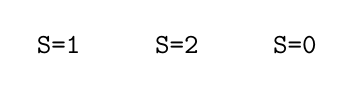
\begin{tikzpicture}
    \coordinate (s0) at (0  cm,0cm);
    \coordinate (s1) at (1.5cm,0cm);
    \coordinate (s2) at (3  cm,0cm);
    \robot{s0}{red};
    \robot{s1}{red};
    \robot{s2}{blue};
    \node[below=of s0]{\texttt{S=1}};
    \node[below=of s1]{\texttt{S=2}};
    \node[below=of s2]{\texttt{S=0}};
  \end{tikzpicture}
  \caption{A diagram of the ternary sensor in which classes are depicted
    as colors. The left red robot detects a kin robot, so its sensor
    returns 1. The middle red robot detects a blue robot, so its sensor
    returns 2. The right robot detects no robot, so its sensor returns
    0.}
  \label{fig:sensor}
\end{figure}
The robots are also equipped with a ternary sensor that is able to
detect the presence of nearby robots and their ``kinness''. Two robots
are \emph{kin} if they belong to the same class (denoted by color in
our experiments); they are \emph{non-kin} otherwise. The sensor is
assumed to have infinite range (we consider non-infinite range in
Sec.~\ref{section:beam_range}). As depicted in Fig.~\ref{fig:sensor},
the sensor returns a reading $S=0$ when no robot is detected, $S=1$
when a kin robot is detected, and $S=2$ when a non-kin robot is
detected. We allow for any number of classes, but the sensor need not
distinguish between different non-kin classes---it only detects
whether a nearby robot belongs to the same class or not.

The objective of our algorithm is to group robots into clusters, such
that all the robots of the same class are packed into one cluster with
no non-kin robots.

\begin{algorithm}[t!]
  \begin{algorithmic}
    \If {$I=0$} \State set wheel speeds to $v_{l_0}$, $v_{r_0}$
    \ElsIf {$I=1$} \State set wheel speeds to $v_{l_1}$, $v_{r_1}$
    \Else \State set wheel speeds to $v_{l_2}$, $v_{r_2}$
    \EndIf
  \end{algorithmic}
  \caption{Controller Design}
  \label{alg:controller}
\end{algorithm}

The controllers we use in our experiments are of the same form as in
\cite{gauci_self-organized_2014}. The controller maps each of the
three sensor values to a set of wheel speeds. Pseudo-code for the
controller is shown in Algorithm \ref{alg:controller}. This controller
has six parameters:

$$[\,v_{l_0}, v_{r_0}, v_{l_1}, v_{r_1}, v_{l_2}, v_{r_2}\,]$$

Keeping with the form used in \cite{gauci_self-organized_2014}, we let these parameters range from -1 to 1. In simulation, we then scale this parameter to range from \SI{-20}{\centi\meter\per\second} to \SI{20}{\centi\meter\per\second}.

  \subsection{Simulation Environment}

    We use the ARGoS simulation environment to search for controller parameters and evaluate them, which has the advantage of allowing us to run trials much faster than on real robots \cite{pinciroli_argos:_2012}. In our simulations, we use a range-and-bearing sensor to implement the theoretical line-of-sight sensor. In our analysis, we describe the sensor as infinitely thin, but in practice it must have some small finite angle. We explore the performance effect of various beam angles in Section \ref{section:beam_angle}. In our simulations, we consider robots to be connected in a cluster if the gap between them is \SI{5}{\centi\meter} or less. This detail is required for the cluster metrics. We now describe how we found these parameters with a grid search.

  \subsection{Cost Functions}

    As with any optimization algorithm, it is important to have a cost function that accurately assigns cost to behaviors. The cost metric that we used (Equation \eqref{eq:cluster_cost}) is based on the cluster metric $c_{\text{gauci}}^{(t)}$ used by \cite{gauci_self-organized_2014}, which is the proportion of the number of robots in the largest cluster to the total number of robots at some time step $t$.

    \begin{equation} \label{eq:cluster_cost}
      c_{\text{total}} =  \frac{1}{n}\sum^n\sum_{t=0}^{T-1} -t c_{\text{gauci}}^{(t)}
    \end{equation}

    Let $n$ be the number of classes of robots, and $T$ be the total number of time steps in the trial being evaluated. We apply this cost function for each class of robots and sum the cluster-metric cost for each class to get the total cost. The negative sign is present because the cluster metric is 0 when no robots are connected and 1 when all robots in a class are connected, so the negative sign assigns more connections a lower cost. We used this cost function in grid search and all following experiments.

    In our experiments, we found that this cost function correctly assigns cost in most scenarios, but it is not ideal because it considers a straight line of robots to be one cluster. For some tasks such as task allocation, we might care about how tightly the swarm is packed in its clusters.

  \subsection{Grid Search}

    In order to exhaustively search the space of possible controllers, we conducted a grid search of the 6-dimensional parameter space. Due to limited computational resources, we were only able to search with a resolution of 7 values per parameter, which means in total we evaluated $7^6=117649$ parameter sets. For each parameter set, we ran 1 trial in 38 different initial configurations, with 100 seconds for each simulation. These initial configurations consisted of uniformly random placement, clusters, and lines of robots distributed throughout the environment. We chose to include some structure configurations (clusters and lines) because we discovered that they varied significantly in performance from uniform random configurations, and by explicitly evaluating on structure configurations we can speak more confidently about the ability of the controller to succeed in any configuration. Otherwise, we would need to have far more trials with uniformly random robot placement to make the same claims. We were able to parallelize across the 38 configurations and run at 75x real time, so it took approximately 5 days to evaluate all the controllers.

    Because the search space is six-dimensional, we chose to visualize it by plotting every pair of parameters against each other. For example, we consider how the cost changes as $v_{l_0}$ and $v_{r_0}$ change. We note that these graphs, shown in Appendix \ref{section:grid_search_images}, show very similar patterns to the same plots presented by \cite{gauci_self-organized_2014}. As an example of reading these plots, we can tell from the plot of parameters 2 and 3 ($I=1$) that there were no good controllers where the left and right wheel speeds were equal and negative (dark squares in the upper left), and that the best controllers had slightly unequal values close to 1 (lightest squares in the bottom left). These plots also visualize how there are some sharp discontinuities where performance changes dramatically.

\section{The Emergent Behavior}

    After running the grid search, the controller with the lowest average cost over all 38 configurations was [1, -$\sfrac{2}{3}$, $\sfrac{1}{3}$, 1, 1, 0]. The resulting behavior is to turn away from kin but turn the opposite way when they see nothing or non-kin. This behavior causes the kin robots to zig-zag in a line towards their kin, and when multiple robots execute this behavior the kin robots form rings. An example of this can be seen in Figure \ref{fig:rings}. Rarely, the robots form shrimp-like shapes which can also be seen in Figure \ref{fig:rings}.

    \begin{figure}
      \centering
      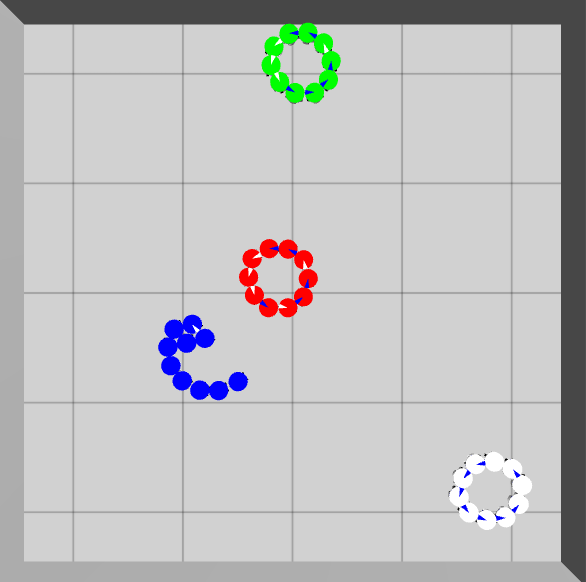
\includegraphics[width=0.5\linewidth]{./images/rings_example.png}
      \caption{the emergent behavior is rings of kin. These rings expand and drift over time.}
      \label{fig:rings}
    \end{figure}

    It's important to note that although we originally hoped that segregated clusters would be tightly packed, in our comprehensive grid search we never found any controller that was capable of this. Another important emergent behavior is that the rings expand over time. When we placed many kin robots together in a large area, they would quickly form a ring and this ring would slowly expand in radius, seemingly infinitely. Explaining or proving this formally is left for future work.

    The dynamics of the robots is far more complex than merely forming rings. A complete description of the observed behavior is beyond the scope of this paper, but we encourage the reader to view the supplementary videos at \href{https://www.youtube.com/playlist?list=PL9HqYJ1IkIKVX9EsT5BY9LnBsBPTjc5bB}{https://goo.gl/z8UAuB}. For example, we notice that the rings, once formed, expand over time. If a ring is disturbed by non-kin robots that trying to pass through, the ring is disrupted and eventually reforms.

\section{Controller Analysis}

  We found from grid search that the parameters [$1$, $-0.6667$, $0.3333$, $1.0$, $1.0$, $0.0$] best achieve segregation as defined by our cluster metric cost function. The actual wheel speeds, which are scaled by $0.2$ to convert to \SI{}{\meter\per\second} are therefore [$0.2$, $-0.1333$, $0.06667$, $0.2$, $0.2$, $0.0$]. Now that we have found parameters that achieve what we consider segregation, we define the conditions under segregation is guaranteed. We first define the conditions under which a kin robot will aggregate with a static kin or ring of kin. We then show that a robot also aggregates to a non-kin. However, we show that aggregation to kin is always faster than aggregation to non-kin. These three proofs partially explain why segregation occurs.

  In all of these proofs we will consider the controller found via grid search since it is the best controller. We also assume the controllers are in sync, which means that each motion is executed for the same $\Delta t$ starting at the same point in time, and that all robots have a fixed positive interwheel distance $W$ and radius $r$.

  \subsection{Aggregation with Kin}

    \begin{figure}[t!]
      \centering
      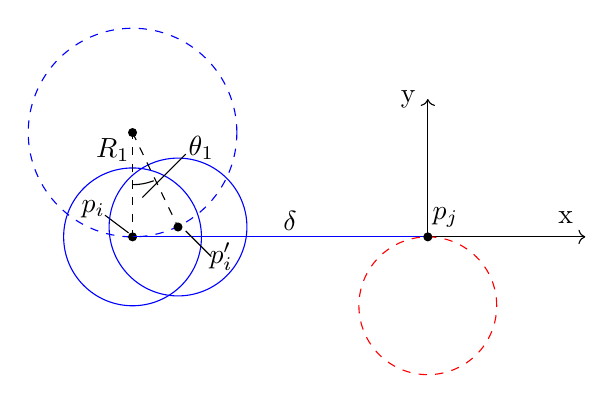
\begin{tikzpicture}[scale=25.0]
        \draw[->] (0.15,0) -- (0.23,0);
        \node at (0.22,.01) {x};
        \draw[->] (0.15,0) -- (0.15,0.07);
        \node at (.14,0.07) {y};

         % c_i
        \filldraw (0,0.053) circle (.002);
        \draw[blue, dashed] (0,0.053) circle (0.053);

         % p_i
        \filldraw (0,-0.0) circle (.002);
        \draw[blue] (0,-.0) circle (0.035);
        \node at (-0.01,.044) {$R_1$};
        \draw[dashed] (0,0.054) -- (0,0.0);
        \draw (-0.014,0.011) -- (-.002,.002);
        \node at (-0.020,0.014) {$p_i$};

        % delta
        \draw[blue] (0,.0) -- (.15,.0);
        \node at (0.08, 0.008) {$\delta$};

         % p'_i
        \filldraw (0.0231,0.005) circle (.002);
        \draw (0.027, 0.003) -- (.04,-0.010);
        \draw[blue] (0.0231,0.005) circle (0.035);
        \draw[dashed] (0,0.053) -- (0.0231,0.005);
        \node at (0.045,-.010) {$p'_i$};

         % p_j
        \draw[dashed, red] (0.15, -0.035) circle (0.035);
        \filldraw (0.15, 0.0) circle (.002);
        \node at (0.159, 0.010) {$p_j$};

        % theta
        \draw (0,.0265) arc [radius=.03, start angle=-90, end angle=-69];
        \node at (.035,.045) {$\theta_1$};
        \draw (.005, .020) -- (.027,.042);

      \end{tikzpicture}
      \caption{The configuration of a robot aggregating to another kin. $R_1$ is the radius of the robots path around the ICC.}
      \label{fig:kin_aggregation}
    \end{figure}

    Imagine an isolated kin robot, $i$ which has sensed another kin or a static ring of kin (kin entity), $j$. This scneario is depicted in Figure \ref{fig:kin_aggregation}. We can define the conditions under which robot $i$ is guaranteed to be closer to the point where the imaginary sensor beam meets the kin entity. This point is chosen as the origin. When robot $i$ starts at $p_i$ with sensor reading $I=1$, it then executes $v_{l_1} = 0.06667$ and $v_{r_1} = 0.2$ and arcs with radius $R_1$ counterclockwise and ends up at position $p'_i$. The condition we need to satisfy is shown in Equation \eqref{eq:generic_agg}.

    \begin{equation} \label{eq:generic_agg}
      \lVert p'_i - p_j \rVert < \lVert p_i - p_j \rVert
    \end{equation}

    We can expand Equation \eqref{eq:generic_agg} and derive a simple condition which describes for which values of $r$, $r_j$, $W$, $\Delta t$ aggregation is guaranteed. The full derivation can be found in Theorem \ref{thm:aggregation_with_kin}, and the result is shown in Equation \eqref{eq:kin_agg_result}. The variable $r_j$ denotes the radius of the kin entity, whereas $r$ still refers to the radius of the single robot $i$.

    \begin{equation} \label{eq:kin_agg_result}
      -\sqrt{r^2+2rr_j}\sin\bigg(\frac{2\Delta t}{15W}\bigg) - W\cos\bigg(\frac{2\Delta t}{15W}\bigg) + W < 0
    \end{equation}

    One can substitute in the parameters of their robot into this equation, and if the condition holds true then the behavior described here is guaranteed.

  \subsection{Aggregation with Non-Kin}

    \begin{figure}[t!]
      \centering
      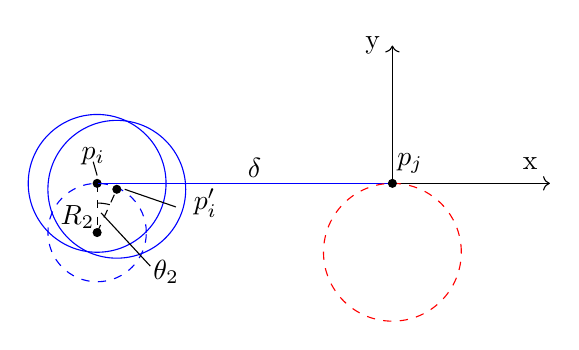
\begin{tikzpicture}[scale=25.0]
        \draw[->] (0.15,0) -- (0.23,0);
        \node at (0.22,.01) {x};
        \draw[->] (0.15,0) -- (0.15,0.07);
        \node at (.14,0.07) {y};

         % c_i
        \filldraw (0,-0.025) circle (.002);
        \draw[blue, dashed] (0,-0.025) circle (0.025);

         % p_i
        \filldraw (0,-0.0) circle (.002);
        \draw[blue] (0,-.0) circle (0.035);
        \node at (-0.01,-.017) {$R_2$};
        \draw (-0.002,0.011) -- (0,.004);
        \node at (-0.002,0.014) {$p_i$};

        % delta
        \draw[blue] (0,.0) -- (.15,.0);
        \node at (0.08, 0.008) {$\delta$};

         % p'_i
        \filldraw (0.01,-0.003) circle (.002);
        \draw[blue] (0.01,-0.003) circle (0.035);
        \draw[dashed] (0,-0.025) -- (0.01,-0.003);
        \draw[dashed] (0,0.0)-- (0,-0.025);
        \draw (0.014, -0.003) -- (.04,-0.012);
        \node at (0.055,-.010) {$p'_i$};

         % p_j
        \draw[dashed, red] (0.15, -0.035) circle (0.035);
        \filldraw (0.15, 0.0) circle (.002);
        \node at (0.159, 0.010) {$p_j$};

        % theta
        \draw (0,-.01) arc [radius=.025, start angle=90, end angle=75];
        \node at (.035,-.045) {$\theta_2$};
        \draw (.002, -.015) -- (.027,-.042);

      \end{tikzpicture}
      \caption{The configuration of a robot aggregating to a non-kin. $R_2$ is the radius of the robots path around the ICC.}
      \label{fig:non_kin_aggregation}
    \end{figure}

    This scenario and proof follows the same pattern as with kin, but the resulting condition is slightly different. We can again expand Equation \eqref{eq:generic_agg}, this time with different coordinates for $p'_i$. The full derivation can be found in Theorem \ref{thm:aggregation_with_non_kin}, and the result is shown in Equation \eqref{eq:non_kin_agg_result}.

    \begin{equation} \label{eq:non_kin_agg_result}
      -\sqrt{r^2+2rr_j}\sin\bigg(\frac{2\Delta t}{10W}\bigg) - \frac{W}{2}\cos\bigg(\frac{2\Delta t}{10W}\bigg) + \frac{W}{2} < 0
    \end{equation}

  \subsection{Segregation}

    So far all of the behaviors we have discussed are actually just aggregation behaviors. Here we partially explain why segregation occurs by showing that kin robots aggregate faster than the non-kin robots. To show that non-kin aggregate more slowly than kin, we show that the displacement during their kin step (the arc left with speeds $0.06667, 0.2$) is greater than the displacement during their non-kin step (with speeds $0.2, 0.0$). This proof can be found with Theorem \ref{thm:seg}. Note that we only consider the magnitude of the step, not the direction, so in theory the longer kin step could aggregate less than the shorter non-kin step, but this partially justifies why kin aggregate faster then non-kin.

  \subsection{Application to Real Swarm Robots}

    The above conditions do not hold true for all scenarios (such as those with large $\Delta t$), but we show that they do hold true for a number of popular robots in Table \ref{table:robots}.

    \begin{savenotes}
    \begin{table}
      \centering
      \caption{Aggregation is guaranteed for many differential drive swarm robots. We used $\Delta t=0.1$ here, and assume $r_j=r$}
      \begin{tabular}{|c|c|c|c|c|c|} \hline
        Robot & $r$ (m) & $W$ (m) & Eq \eqref{eq:kin_agg_result}& Eq \eqref{eq:non_kin_agg_result} & Guaranteed \\ \hline
        foot-bot\footnote{\href{https://github.com/ilpincy/argos3/blob/master/src/plugins/robots/foot-bot/simulator/footbot_entity.cpp}{ARGoS file footbot\_entity.cpp}} &
            0.085 & 0.14 & -0.013 & -0.020 & Yes \\ \hline
        Khephera IV\footnote{Khephera IV User Manual, page 66.} &
            0.07 & 0.1054 & -0.014 & -0.021 & Yes \\ \hline
        E-Puck 2\footnote{\href{http://projects.gctronic.com/epuck2/e-puck2-flyer.pdf}{http://projects.gctronic.com/epuck2/e-puck2-flyer.pdf}} &
            0.035 & 0.053 & -0.013 & -0.020 & Yes \\ \hline
        Kilobot\footnote{\href{https://www.k-team.com/mobile-robotics-products/kilobot/specifications}{https://www.k-team.com/mobile-robotics-products/kilobot/specifications}} &
            0.0165 & 0.030\footnote{only approximate} & -0.009 & -0.014 & Yes \\ \hline
      \end{tabular}
      \label{table:robots}
    \end{table}
    \end{savenotes}

    Ultimately, we can use these geometric proof to make useful assertions about the behavior of an individual in our swarm and of the swarm as a whole. While we have not shown that segregation is guaranteed in all cases, this may serve as a building block for more general claims.

\section{Experimental Results}

  \subsection{Comparing Cost Functions} \label{section:evaluating_cost_functions}

    We ran grid search using both of our cost functions.

  \subsection{Scalability Study} \label{section:scalability}

    In this experiment we investigate how segregation behavior scales with the number of classes and number of robots in the environment. We varied the number of classes from 1 to 25 and ran 100 trials of robots uniformly randomly distributed.

    \paragraph{Fixed number of robots per class}

    We first considered having 10 robots for each class. However, this means that in the trial with 25 classes there are 25 times the total number of robots than in the 1-class trial. This means that occlusion of robots is more likely and so the cost increases with more classes. The results of this are plotted in Figure  \ref{fig:num_classes_10}.

    \paragraph{Fixed total number of robots}

    Another scenario is to consider a fixed number of robots and split them into more and more classes. We choose 100 robots because we are still able to get 4 robots per class at 25 classes. As you can see in Figure \ref{fig:num_classes_100}, the cost no longer increases as the number of classes increases. However, the cost for just a few classes is much higher. This is expected, because when there are many robots of a single class, our controller forms very large sparse rings where robots are too far apart to be considered clustered.

    Ultimately, we can say that our controller scales well to many classes of robots, but not very well to many robots.

    \begin{figure}[H]
      \centering
      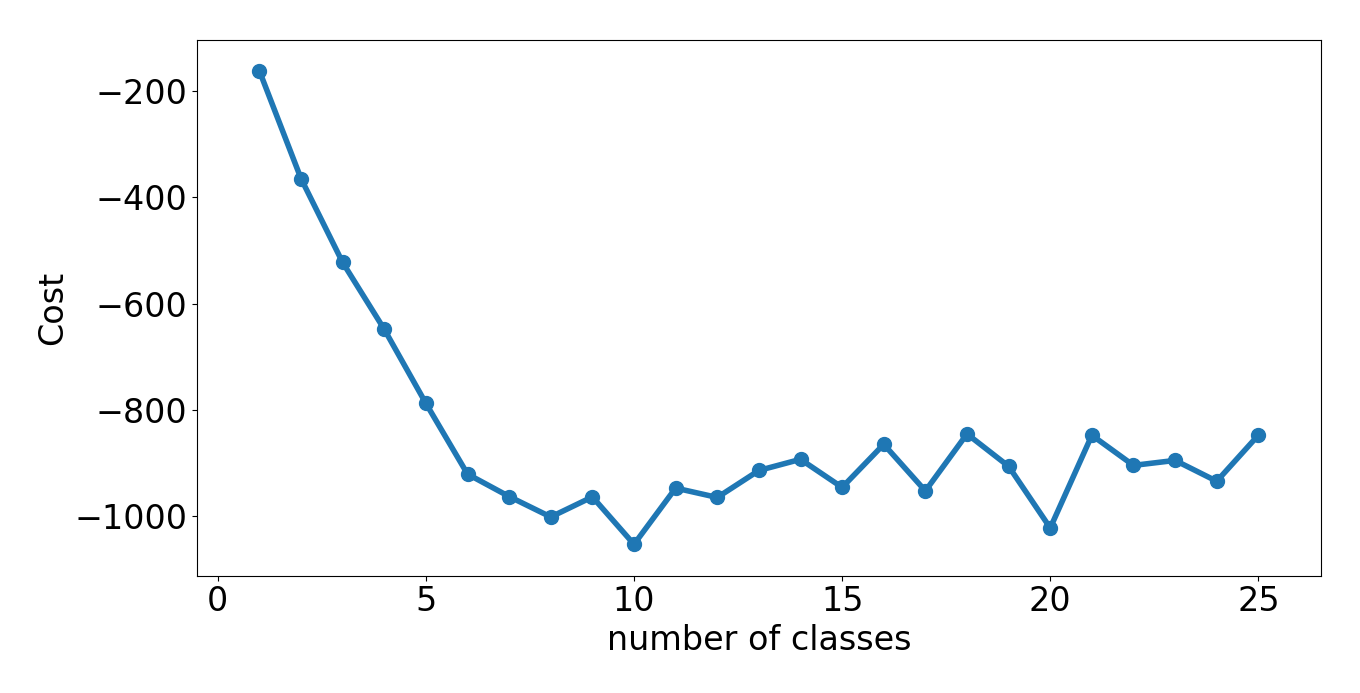
\includegraphics[width=1\linewidth]{./images/num_classes_vs_cost_100_robots.png}
      \caption{The average cost with 100 robots divided into N classes. More classes are lower cost partially because kin robots stay close enough to be considered clusters.}
      \label{fig:num_classes_100}
    \end{figure}

    \begin{figure}[H]
      \centering
      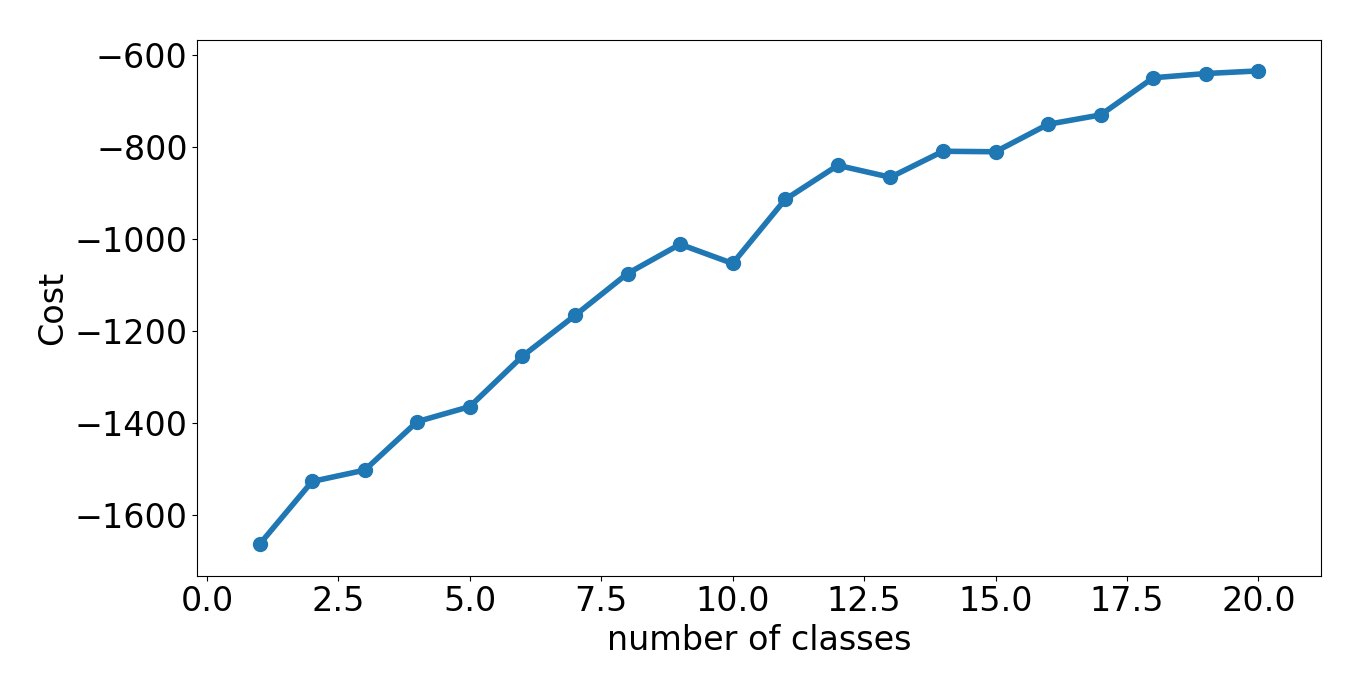
\includegraphics[width=1\linewidth]{./images/num_classes_vs_cost_10_per_class.png}
      \caption{The average cost with N classes, 10 robots per class. More classes are higher cost because other robots obstruct your view making sensing kin less likely.}
      \label{fig:num_classes_10}
    \end{figure}

  \subsection{The Effect of Implementation Details of the sensor} \label{section:sensor_impl}

    We found in our experiments that the implementation details of the line-of-sight sensor have a significant effect on the behavior of the controller.

    Initially, our method for determining sensor state from our simulated range-and-bearing sensors was to consider all the robots within some small angle in front of the robot and pick the closest one. This is very similar to what would be provided by a real-world camera that uses colored skirts on each robot and picks the largest blob as the robot to be detected. This sensor implementation works well and was used in all our genetic algorithm and grid search experiments. However, we found later that if the robots instead always prefer to react to kin over non-kin, you can form larger rings more quickly and robustly. For example, if there are two robots within the field of view of your sensor and the non-kin robot is closer, you will ignore it and execute the $I=1$ state which will drive you towards the farther away kin robot. Exploring exactly which of the various implementation details have what effect on cost is left for future work.

  \subsection{The Effect of the Beam Angle} \label{section:beam_angle}

    On a real robot, there must be some finite beam angle to the theoretically line-of-sight sensor. We ran 100 trials in simulation with uniformly random initial distributions of 40 robots with various half beam angles. Figure \ref{fig:beam_angle} shows the results, as well as a diagram showing how we define half beam angle. The best half beam angle we tested was \ang{15}, and angles smaller or larger became progressively worse. We found that at lower beam angles, it was possible for a robot to become stuck in groups of two or three where the robots spent all their time looking at each other and not peeking around them to find kin. At larger angles, we suspect the behavior fails because larger beam angles cause the rings to enlarge faster, which in turn causes the rings to be so large that they are not considered a cluster anymore and so the cost rises.

    \begin{figure}[H]
      \centering
      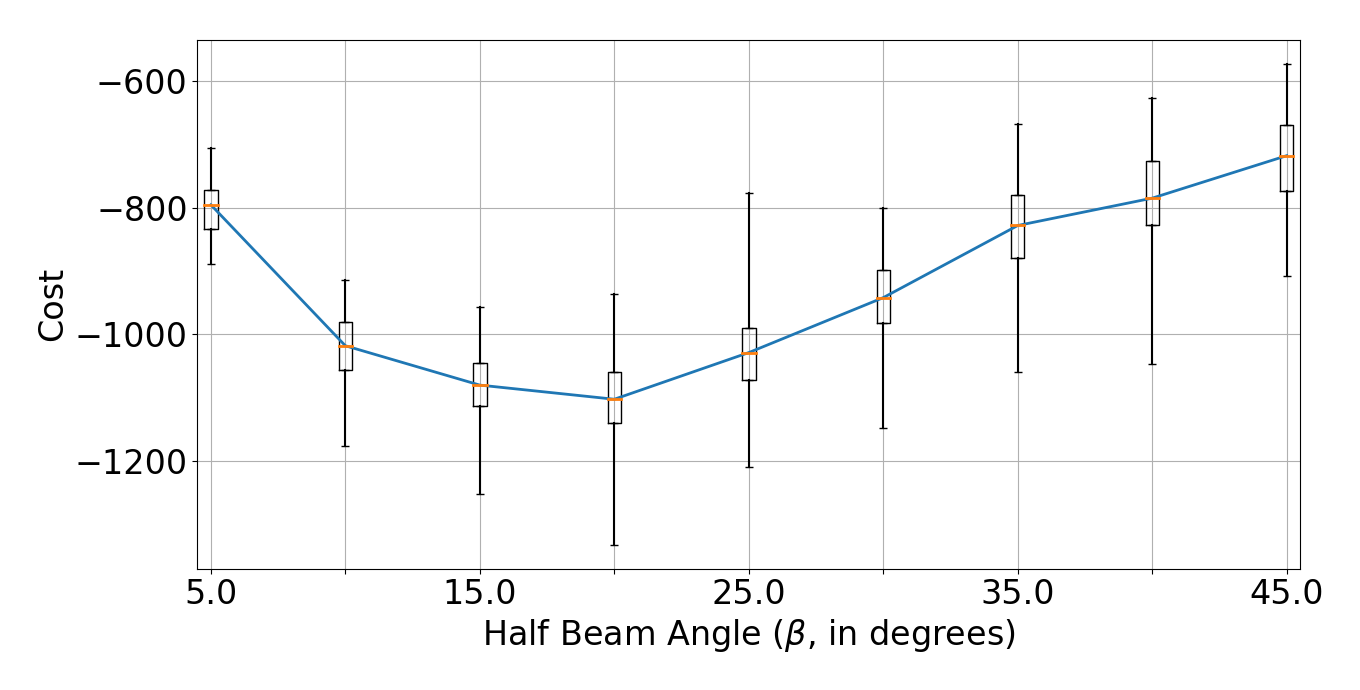
\includegraphics[width=1\linewidth]{./images/beam_angle.png}
      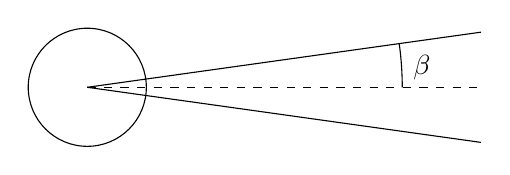
\begin{tikzpicture}
        \draw (0,0) circle (0.75);
        \draw (0,0) -- (5,0.7);
        \draw[dashed] (0,0) -- (5,0);
        \draw (0,0) -- (5,-0.7);
        \draw (4,0) arc [radius=4, start angle=0, end angle=8];
        \node at (4.25,0.25) {$\beta$};
      \end{tikzpicture}
      \caption{A \ang{15} degree half beam angle is best for segregation. Lower cost is better.}
      \label{fig:beam_angle}
    \end{figure}

  \subsection{The Effect of Beam Length} \label{section:beam_range}

    We also consider what happens if our theoretically infinite sensor now has finite range. We use \ang{15} half beam angle and the same experimental setup as with the beam angle experiments. Analogously to \cite{gauci_self-organized_2014}, we consider the maximum range of the sensor as the diagonal length of the square in which the robot are initially distributed. In all our experiments, this square was \SI{5}{\meter} on each side, so we consider a range of \SI{7.07}{\meter} to be effectively unlimited. We report the costs for beam ranges as a fraction of this maximum range. As shown in Figure \ref{fig:beam_range}, a beam range of 35\% of the theoretical maximum performs just as well as an infinite sensor. Below this, the performance degrades. However, even a beam range of 7\% of unlimited is more effective than zero range at segregation.

    \begin{figure}
      \centering
      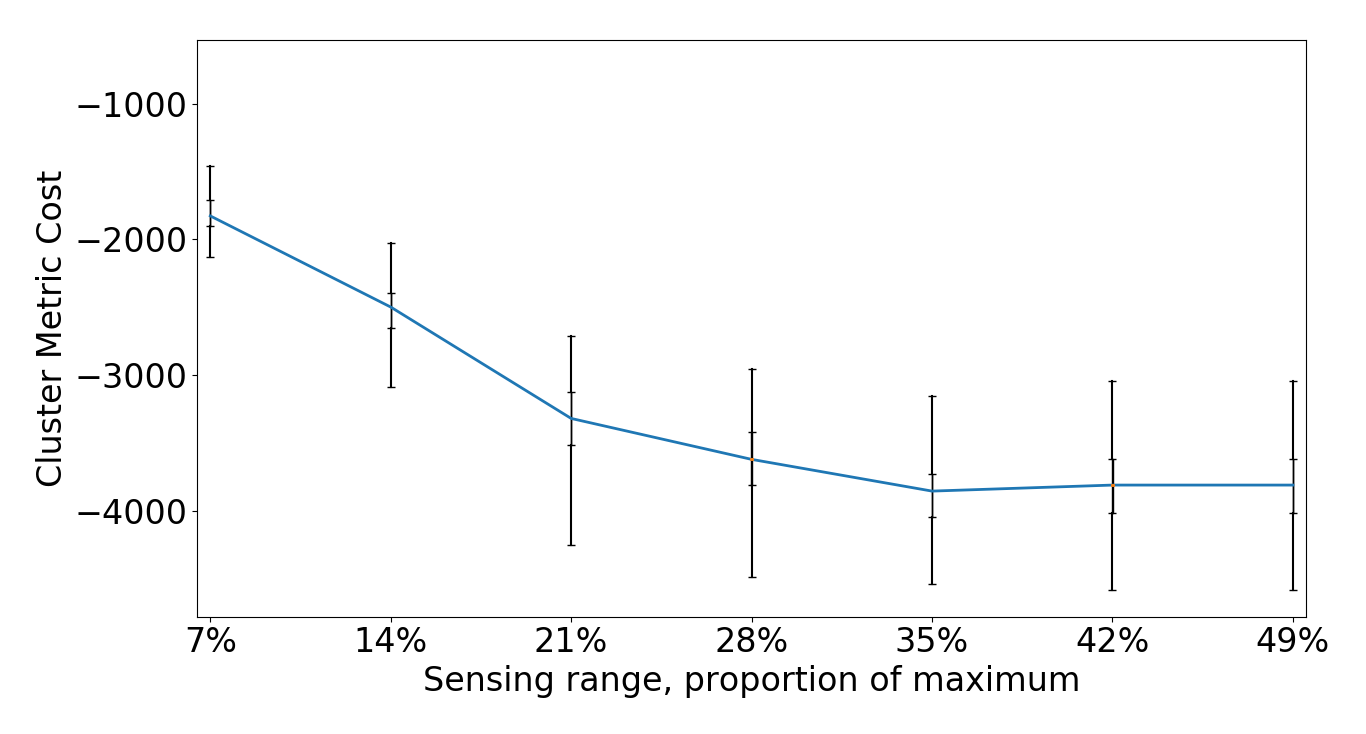
\includegraphics[width=1\linewidth]{./images/beam_length.png}
      \caption{Segregation is robust to very finite sensor beam ranges. The blue bar indicates the worst (highest) attainable cost in which all robots are isolated from any kin.}
      \label{fig:beam_range}
    \end{figure}

\section{Conclusion}

  In this paper, we demonstrate that oblivious robots are capable of $n$-class segregation. We use a simple controller design consisting of a 6-tuple. This controller is invariant to the number of classes, so any given controller can work for any number of classes. We performed a grid search to learn about the full parameter space, and we investigated the effect of sensor implementation details and the number of robots and classes on performance. We find that robust segregation is possible, although not guaranteed. Instead, we prove that kin robots will aggregate, non-kin robots will also aggregate, and kin robots aggregate faster than non-kin robots.

\bibliography{RBE595.bib}
\bibliographystyle{unsrt}

\onecolumn
\appendix
\section{Appendix}


  \begin{theorem} \label{thm:aggregation_with_kin}
    An isolated robot will aggregate to a kin entity.
  \end{theorem}
  \begin{proof}
    Use the differential drive forward kinematics model to determine the coordinates of $p'_i$.
    \begin{align} \label{eq:kin_theta_and_r}
      \theta_1 &= \Delta t\omega = \Delta t \frac{v_{r_1} - v_{l_1}}{W} = \Delta t \frac{0.2 - 0.06667}{W} = \frac{2\Delta t}{15W} \\
      R_1 &= \frac{W}{2}\bigg(\frac{v_{r_1} + v_{l_1}}{v_{r_1} - v_{l_1}}\bigg) = \frac{W}{2}\bigg(\frac{0.2 + 0.06667}{0.2 - 0.06667}\bigg) = W
    \end{align}

    We can define the coordinates of $p_i$, $p_j$, and $p'_i$.

    \begin{align} \label{eq:kin_coordinates}
      p_i &= \begin{bmatrix}-\delta \\ 0\end{bmatrix} \\
      p_j &= \begin{bmatrix}0 \\ 0\end{bmatrix} \\
      p'_i &= \begin{bmatrix}-\delta+R_1\sin(\theta_1) \\ R_1-R_1\cos(\theta_1)\end{bmatrix}
    \end{align}

    We also define the minimum possible $\delta$, which is acheived when the robots and tangent.

    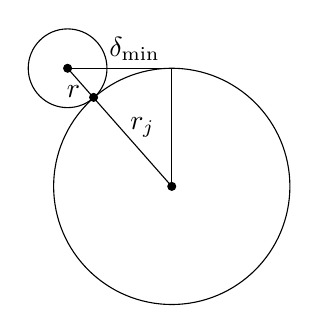
\begin{tikzpicture} [scale=0.5]
      \draw (0,0) circle (1);
      \filldraw (0,0) circle (0.1);
      \node at (0.15,-0.6) {$r$};
      \filldraw (2.6457,-3) circle (0.1);
      \draw (2.6457,-3) circle (3);
      \node at (1.9,-1.5) {$r_j$};
      \draw (2.6457,0) -- (2.6457,-3);
      \filldraw (.66,-.74) circle (0.1);
      \draw (0,0) -- (2.6457,-3);
      \draw (0,0) -- (2.6457,0);
      \node at (1.7,.5) {$\delta_{\text{min}}$};
    \end{tikzpicture}
    \begin{align} \label{eq:min_delta}
      \delta_{\text{min}} = \sqrt{(r + r_j)^2 - (r_j)^2} = \sqrt{r^2 + 2rr_j + r_j^2 - r_j^2} = \sqrt{r^2+2rr_j}
    \end{align}


    Show that $\lVert p'_i - p_j\rVert < \lVert p_i - p_j\rVert$ (Equation \eqref{eq:generic_agg}) for all $\delta > \sqrt{r^2+2rr_j}$.

    \begin{align*}
      \lVert p'_i - p_j \rVert &< \lVert p_i - p_j \rVert \\
      \sqrt{(p'_{ix} - p_{jx})^2 + (p'_{iy} - p_{jy})^2} &< \sqrt{(p_{ix} - p_{jx})^2 + (p_{iy} - p_{jy})^2} \\
      \sqrt{(-\delta+R_1\sin(\theta_1)-0)^2 + (R_1-R_1\cos(\theta_1-0)^2} &< \sqrt{(-\delta-0)^2 + (0-0)^2} \\
      \sqrt{\delta^2-2\delta R_1\sin(\theta_1) + R_1^2\sin(\theta_1)^2 + R_1^2-2R_1^2\cos(\theta_1)+R_1^2\cos(\theta_1)^2} &< \delta \\
      \intertext{Apply $\sin^2+\cos^2=1$}
      \sqrt{\delta^2-2\delta R_1\sin(\theta_1) + 2R_1^2-2R_1^2\cos(\theta_1)} &< \delta \\
      \delta^2-2\delta R_1\sin(\theta_1) + 2R_1^2-2R_1^2\cos(\theta_1) &< \delta^2 \\
      -\cancel{2}\delta \cancel{R_1}\sin(\theta_1) - \cancel{2}R_1^{\cancel{2}}\cos(\theta_1) + \cancel{2}R_1^{\cancel{2}} &< 0 \\
      -\delta \sin(\theta_1) - R_1\cos(\theta_1) + R_1 &< 0 \\
      \intertext{We assume $\theta_1\in(0,\sfrac{\pi}{2})$, so if the above condition holds for the smallest $\delta=\delta_{\text{min}}$, it holds for greater $\delta$.}
      -\sqrt{r^2+2rr_j}\sin\bigg(\frac{2\Delta t}{15W}\bigg) - W\cos\bigg(\frac{2\Delta t}{15W}\bigg) + W &< 0
    \end{align*}
  \end{proof}

  \begin{theorem} \label{thm:aggregation_with_non_kin}
    An isolated robot will aggregate to a non kin entity.
  \end{theorem}
  \begin{proof}
    \begin{align}
      \begin{split} \label{eq:non_kin_theta_and_r}
        \theta_2 &= \Delta t\omega = \Delta t \frac{v_{r_2} - v_{l_2}}{W} = \Delta t \frac{0.2 - 0.0}{W} = \frac{2\Delta t}{10W} \\
        R_2 &= \frac{W}{2}\bigg(\frac{v_{r_2} + v_{l_2}}{v_{r_2} - v_{l_2}}\bigg) = \frac{W}{2}\bigg(\frac{0.2 + 0.0}{0.2 - 0.0}\bigg) = \frac{W}{2}
      \end{split}
    \end{align}

    We can define the coordinates of the new $p'_i$.

    \begin{align} \label{eq:non_kin_coordinates}
      p'_i = \begin{bmatrix}-\delta+R_2\sin(\theta_2) \\ -R_2+R_2\cos(\theta_2)\end{bmatrix}
    \end{align}

    Show that $\lVert p'_i - p_j\rVert < \lVert p_i - p_j\rVert$ for all $\delta > \sqrt{r^2+2rr_j}$. This follows the same steps as the Theorem \ref{thm:aggregation_with_kin}.

    \begin{align*}
      \lVert p'_i - p_j \rVert &< \lVert p_i - p_j \rVert \\
      \sqrt{(-\delta+R_2\sin(\theta_2)-0)^2 + (-R_2+R_2\cos(\theta_2-0)^2} &< \sqrt{(-\delta-0)^2 + (0-0)^2} \\
      \sqrt{\delta^2-2\delta R_2\sin(\theta_2) + R_2^2\sin(\theta_2)^2 + R_2^2-2R_2^2\cos(\theta_2)+R_2^2\cos(\theta_2)^2} &< \delta \\
      \sqrt{\delta^2-2\delta R_2\sin(\theta_2) + 2R_2^2-2R_2^2\cos(\theta_2)} &< \delta \\
      -2\delta R_2\sin(\theta_2) - 2R_2^2\cos(\theta_2) + 2R_2^2 &< 0 \\
      -\delta \sin(\theta_2) - R_2\cos(\theta_2) + R_2 &< 0 \\
      \intertext{We assume $\theta_2\in(0,\sfrac{\pi}{2})$, so if the above condition holds for the smallest $\delta=\delta_{\text{min}}$, it holds for greater $\delta$.}
      -\sqrt{r^2+2rr_j}\sin\bigg(\frac{2\Delta t}{10W}\bigg) - \frac{W}{2}\cos\bigg(\frac{2\Delta t}{10W}\bigg) + \frac{W}{2} &< 0
    \end{align*}
  \end{proof}

  \begin{theorem} \label{thm:seg}
    The distance moved in the kin step is always greater than the distance moved in the non-kin step.
  \end{theorem}
  \begin{proof}
    We compare the arc lengths derived from the wheels speeds.
    \begin{align*}
      \theta_1 R_1 &> \theta_2 R_2 \\
      \frac{2\cancel{\Delta t}}{15\cancel{W}} \cancel{W} &> \frac{\cancel{2}\cancel{\Delta t}}{10\cancel{W}} \frac{\cancel{W}}{\cancel{2}} \\
      \frac{2}{15} &> \frac{1}{10} \\
    \end{align*}
  \end{proof}

  \subsection{Grid Search Images} \label{section:grid_search_images}

    \begin{figure}[H]
      \centering
      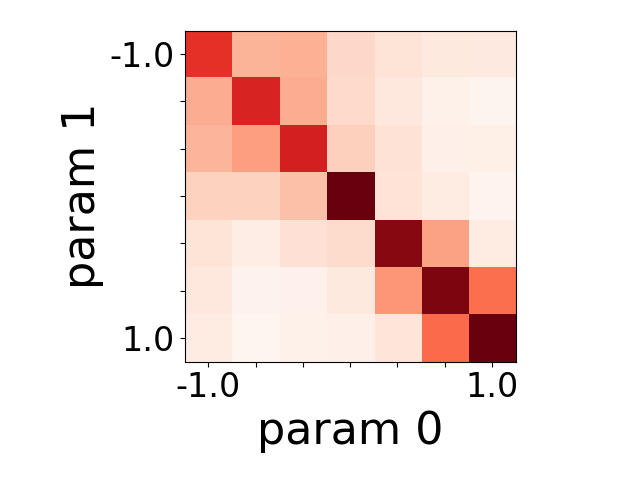
\includegraphics[width=0.29\linewidth]{./images/0_1_grid_img.png}
      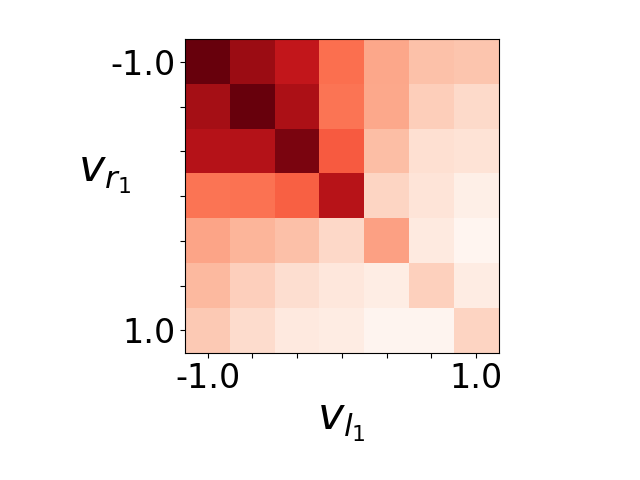
\includegraphics[width=0.29\linewidth]{./images/2_3_grid_img.png}
      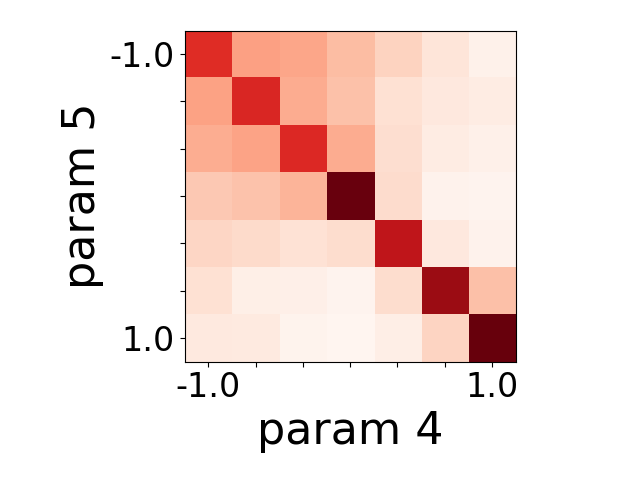
\includegraphics[width=0.29\linewidth]{./images/4_5_grid_img.png}
      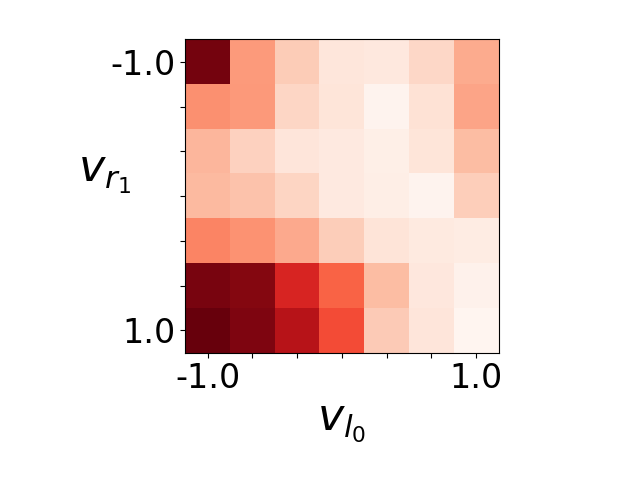
\includegraphics[width=0.29\linewidth]{./images/0_3_grid_img.png}
      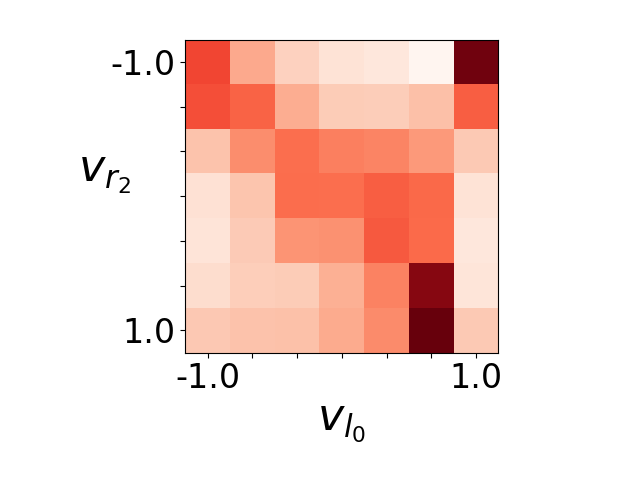
\includegraphics[width=0.29\linewidth]{./images/0_5_grid_img.png}
      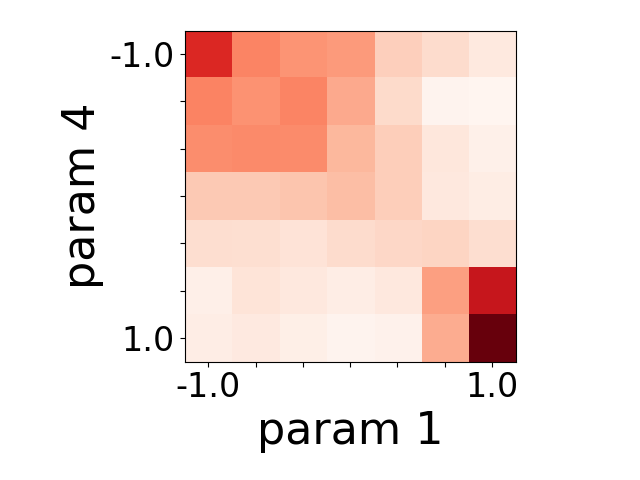
\includegraphics[width=0.29\linewidth]{./images/1_4_grid_img.png}
      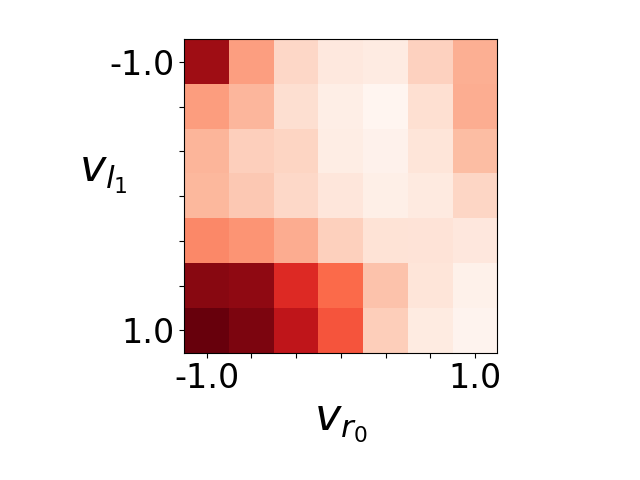
\includegraphics[width=0.29\linewidth]{./images/1_2_grid_img.png}
      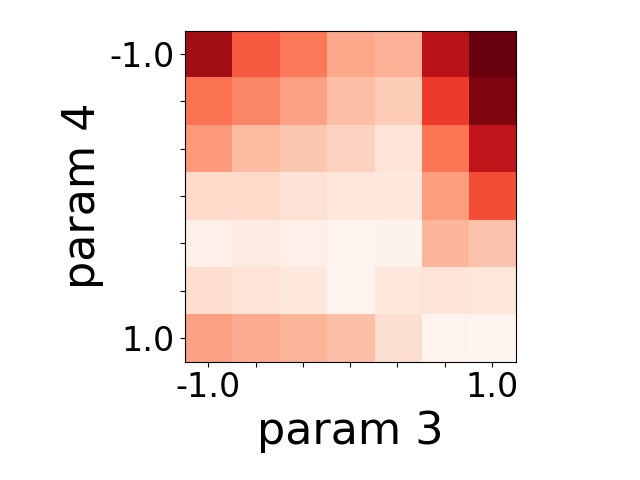
\includegraphics[width=0.29\linewidth]{./images/3_4_grid_img.png}
      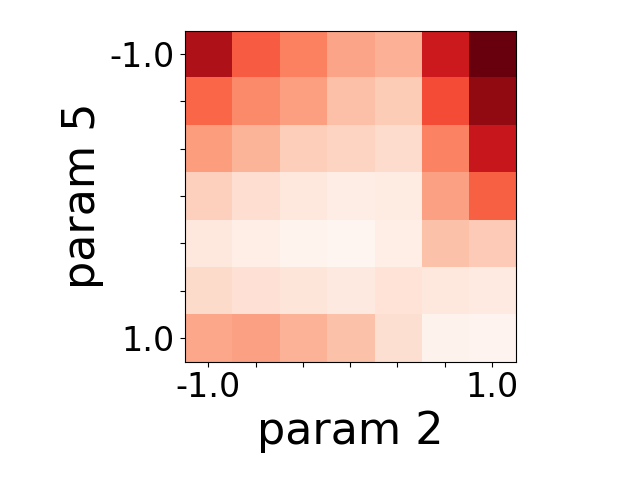
\includegraphics[width=0.29\linewidth]{./images/2_5_grid_img.png}
      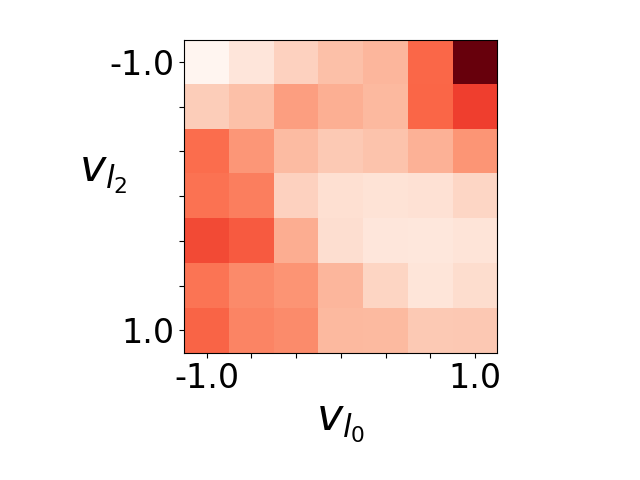
\includegraphics[width=0.29\linewidth]{./images/0_4_grid_img.png}
      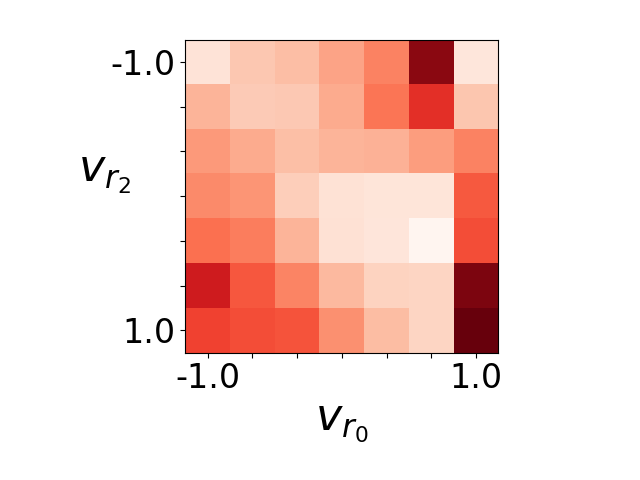
\includegraphics[width=0.29\linewidth]{./images/1_5_grid_img.png}
      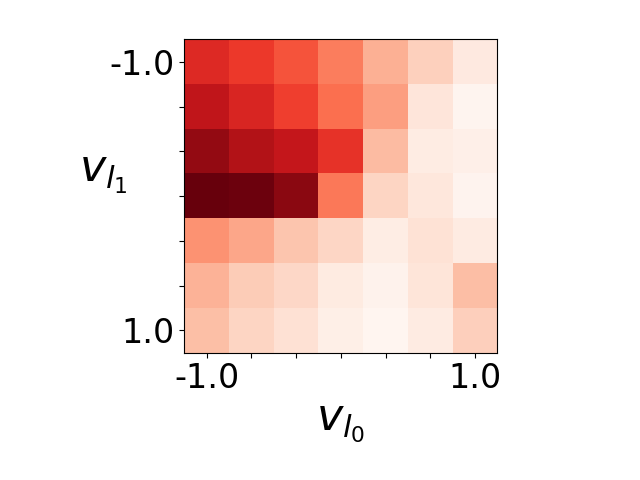
\includegraphics[width=0.29\linewidth]{./images/0_2_grid_img.png}
      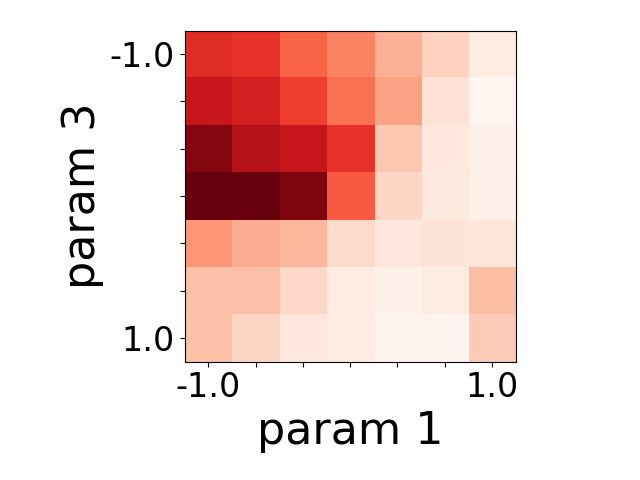
\includegraphics[width=0.29\linewidth]{./images/1_3_grid_img.png}
      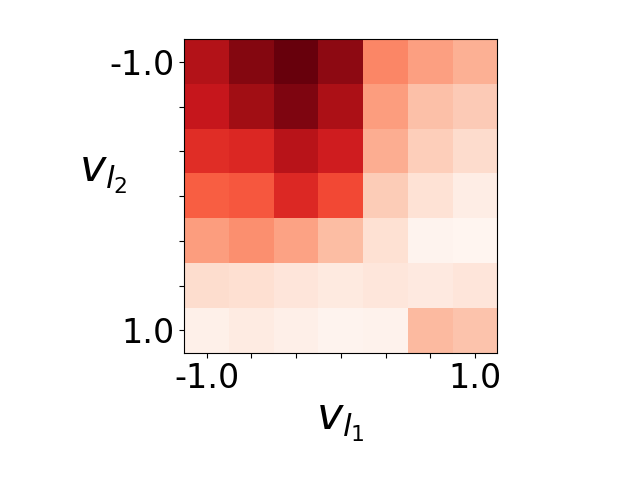
\includegraphics[width=0.29\linewidth]{./images/2_4_grid_img.png}
      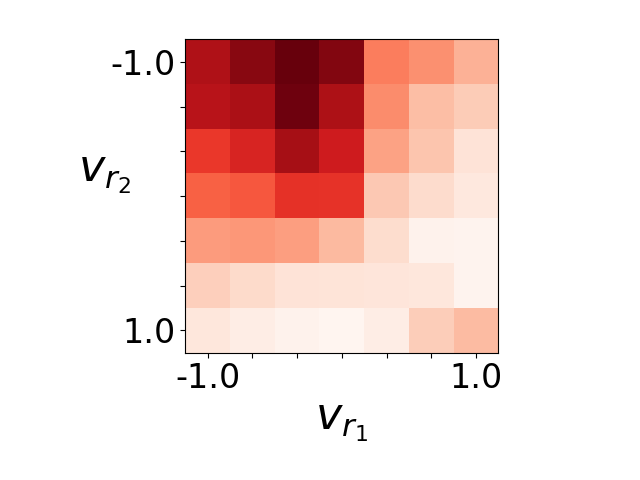
\includegraphics[width=0.29\linewidth]{./images/3_5_grid_img.png}
      \caption{Each grid cell shows the cost of the best controller with the x-axis and y-axis parameters at that given cell value.}
    \end{figure}


\end{document}
